\documentclass[10pt]{article}
\usepackage[utf8]{inputenc}

\usepackage{booktabs, multicol, makecell, amsmath, adjustbox}
\usepackage{graphicx, tikz,tabularx}
\usepackage{subcaption}
\usetikzlibrary{shapes.geometric, matrix,arrows,positioning,calc,intersections}

\title{Optimum design of laminated composites for minimum thickness by a variant
of genetic algorithm}

\begin{document}

\begin{titlepage}
	\maketitle
\end{titlepage}

\begin{titlepage}
	\begin{abstract}
		Traditionally, classic lamination theory is widely used to compute
properties of composite materials under in-plane and out-of-plane loading from
a knowledge of the material properties of the individual layers and the
laminate geometry. In this study, a systematic procedure is proposed to design
an artificial neural network for a practical engineering problem, which is
applied to calculate the strength ratio of a laminated composite material under
in-plane loading, in which the genetic algorithm is proposed to optimize the search
process at four different levels: the architecture, parameters, connections of
the neural network, and active functions. 

	\end{abstract}
\end{titlepage}


\section{Introduction}
Composite materials offer improved strength, stiffness, corrosion resistance,
etc. over conventional materials, and are widely used as alternative materials
for applications in various industries ranging from electronic packaging to golf
clubs, and medical equipment to homebuilding, making aircraft structure to space
vehicles. The stacking sequence and fiber orientation of composite laminates
give the designer additional degree of freedom to tailor the design with
respect to strength or stiffness.  One widely known advantage of using composite
material is can significantly reducing the weight of target structure, and many
researchers attempted to improve the efficiency of using composite material by
minimizing the thickness\cite { schmit1973optimum, schmit1977optimum,
	fukunaga1991strength, soares1995discrete, le1995improved,
	jayatheertha1996application, wang1996optimum, adali1997minimum,
	correia1997higher, scares1997optimization, abu1998optimum, lombardi1998anti,
	le1998design, sivakumar1998optimum, barakat1999use, richard2000reliability,
moita2000sensitivity, soremekun2001composite, walker2003technique,
di2003multiconstrained, kere2003using}.

In practice, fiber orientations are restricted to a finite set of angles and
ply thickness is a specific numeric value.  Because the design variables are
not continueous, a gradient-based optimization procedure, such as the gradient
descent method, is not suitable to cope with such problems.  Moreover, gradient-based
optimization approach is very easily to get trapped in local minima, and
many local optimum may exist in structural optimization problems. A stochastic
optimization, such as the genetic algorithm(GA) and simulated annealing(SA), can
deal with optimization problems with discrete variables. Besides, the stochastic
method could escape from the local optimum, and obtain the global optimum.  GA is one of
the most reliably stochastic algorithms, which has been widely used in solving
constraint design for composite
laminate\cite{callahan1992optimum,soremekun2001composite,park2001stacking,walker2003technique,deka2005multiobjective,pelletier2006multi,jadhav2007parametric,kim2007development,park2008improved}.
Although GA gains different advantages for solving discrete problems, many
disadvantages exist within this approach. First, the optimization process of GA
parameters, such as the population size, parent population,mutation percentage,
etc., is very tedious; Second, the GA needs to evaluate the objective functions
many times to achieve the optimization, and the computation cost is very high;
the last problem within GA is the premature convergence. GA consists of five
basic parts: the variable coding, selection scheme, crossover operator, mutation
operator, and how the constraints are handled.

The first issue when implementing a GA is the representation of design
variables, and an appropriate design representation is crucial to enhance the
efficiency of GA. The canonical GA has always used binary strings to encode
alternative solutions, however, some argued that the minimal cardinality, i.e.,
the binary representation, is not the best option. 

Selection scheme plays a critical role in balancing the dilemma of exploration
and exploitation inherent in GA, and various selection methods, for example,
roulette wheel, elitist, and tournament, etc. have been proposed to overcome
this issue. Both roulette selection and tournament selection are well-studied
and widely employed in the optimization design of laminated composite due to
their simplicity to code and efficiency for both nonparallel and parallel
architectures.

Crossover is another crucial operator introduced into the GA
methodology framework, in which the alternative solution is generated from the
mating pool.  multiple types of crossover operator have been utilized in the optimization
design of composite structures, such as, one-point, two-point, and uniform
crossover.

GA is originally proposed for unconstrained optimization. However, in order to
deal with constrained design for composite laminate, some techniques were
introduced into the GA. The first method is using of data structure, special
data structure was developed to fulfill the symmetry constraint of the laminate,
which consists of coding only half of the laminate and considering that each
stack of the laminate is formed by two laminae with the same orientation but
opposite signs\cite{le1995improved,kogiso1994design}. A penalty function is
developed to convert a constrained problem into an unconstrained problem by
adding a penalty term to the objective function. Another method to solve the
constrained problem is introducing repair strategy by Todoroki and Haftka
\cite{todoroki1998stacking}, which is aim to transform infeasible solutions to
feasible solution by incorporating problem-specific knowledge. 

Another major concern within GA is the convergence speed in terms of the time
and computation cost needed to reach a solution of desired quality. The
objective function based on the CLT is excessively time-consuming and complicate
to evaluate, besides, the target function of GA  needs to calculate many
times. The traditional method to deal with this issue is by increasing the
selection pressure to accelerate the convergence speed, however, in some cases,
this approach does not achieve an ideal result. Because the GAs just provides a
methodological framework to deal with tricky problems, which is heavily
inspired by evolution of biology, it is unnecessary to exactly follow all the
GA operation. It is possible to just perform one or more GA operations, and
incorporate other techniques into GA. In the present study, a variant of mutation
operator is introduced to accelerate the convergence process.
  

To check the feasibility of a laminate composite by imposing a strength
constraint, various failure criterion have been proposed to decide whether it
fails or not, such as  maximum stress failure theory, maximum strain failure
theory, Tsai-Hill Failure theory, and Tsai-Wu criterion. Each theory is proposed
based on massive experiment data or complicate mathematical model, however
single use any of them may lead to a false optimum design for some loading case
due to the particular shape of its failure envelope. In order to overcome this
disadvantage within every failure theory, two reliably failure criteria, maximum
stress theory and Tsai-wu criterion are employed to check whether the composite
laminate fullfills the constraint.

The rest of the paper is organized as follows. Section 2 explains the classical laminate theory and
the failure criteria taken in the present study.  Section 3 explains the proposed method of
selection strategy and self-adaptative parameters for mutation during the GA process. Section 4
describes the result of the numerical experiments in different cases, and in the conclusion section,
we dicuss the results.



\section{Introduction}
Fiber-reinforced composite materials have been widely used in many industries
because they offer improved mechanical stiffness, strength, and low specific
gravity of fibers  over conventional materials. The use of composite material
materials in structural application is range from electronic packaging, sports
equipment, homebuilding, medical prosthetic devices, to high performance
military structures. The stacking sequence, ply thickness, and fiber
orientation of composite laminates give the designer additional ’degree of
freedom’ to tailor the design with respect to strength or stiffness. Classic
lamination theory(CLT) is taken to predict the behavior of a laminate from a
knowledge of the composite laminate properties of the individual layers and the
laminate geometry.

Evolutionary artificial neural networks(EANN's) is a special class of artifical
neural networks(ANN's) in which evolutionary algorithms(ES's) are introduced to
learn the optimal ANN. EA's can be used in the ANN at three different levels:
connection weights, architectures, input features, and learning rules. It is
shown, the combinations of ANN's and EA's can significantly improve the
performance of intelligent systems that rely's on ANN's or EA's alone.



The rest of the paper is organized as follows. Section 2 explains the classical
laminate theory and the failure criteria taken in the present study. Section 3
explains the design of artifical neural network for mathmatical model
approximation.  Section 4 reviews the use of genetic algorithm in the design of
neural network architecture and the parameters optimization during the training
process of neural network.  design Section 4 describes the result of the
numerical experiments in different cases, and in the Conclusion section we
dicuss the results.
\section{Classic Lamination Theory}
Classical lamination theory is based upon three simplifying engineering
assumptions: (1) Each layer's thickness is very small and consist of
homogeneous, orthotropic material, and these layers are prefectly bonded
together; (2) The entire laminated composite is supposed to be under plane
stress; (3) Normal cross sections of the entire laminate is normal to the
deflected middle surface, and do not change in thickness.
\begin{figure}
\centering
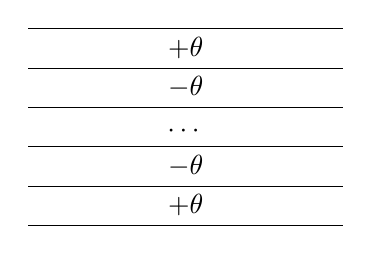
\begin{tikzpicture}
	\draw (0,0) -- (4,0);
	\draw (0,-0.5) -- (4,-0.5) node[midway, above] {$\mathit{+}\theta$};
	\draw (0,-1) -- (4,-1) node[midway, above] {$\mathit{-}\theta$} ;
	\draw (0,-1.5) -- (4,-1.5) node[midway, above] {$\cdots$};
	\draw (0,-2) -- (4,-2) node[midway, above] {$\mathit{-}\theta$};
	\draw (0,-2.5) -- (4,-2.5) node[midway, above] {$\mathit{+}\theta$};
\end{tikzpicture}
\caption{Model for Angle ply laminate}
\end{figure}

\subsection{Stress and Strain in a Lamina}
For a single lamina has a small thickness under plane stress, and it's upper and lower surfaces of the lamina are
free from external loads. According to the Hooke's Law, the three-dimensional stress-strain equations can be reduced to
two-dimensional stress-strain equations. The stress-strain relation in local axis 1-2 is:
\begin{equation}
    \begin{bmatrix}
        \sigma _1\\
        \sigma _2\\
        \tau_{12}
    \end{bmatrix}
    =
    \begin{bmatrix}
        Q_{11} & Q_{12} & 0\\
        Q_{12} & Q_{22} & 0\\
        0      &  0     & Q_{66}
    \end{bmatrix}
    \begin{bmatrix}
        \varepsilon_1\\
        \varepsilon_2\\\gamma_{12}
    \end{bmatrix}
\end{equation}
where $Q_{ij} $are the stiffnesses of the lamina that are related

to engineering elastic constants given by
\begin{equation}
    \begin{split}
    &Q_{11}=\frac{E_1}{1-v_{12}v_{21}}\\
    &Q_{22}=\frac{E_2}{1-v_{12}v_{21}}\\
    &Q_{66}=G_{12}\\
    &Q_{12}=\frac{v_{21}E_2}{1-v_{12}v_{21}}\\
    \end{split}
\end{equation}

where $E_1, E_2, v_{12}, G_{12} $ are four independent engineering elastic constants, which are defined as follows: $E_1 $ is the longitudinal Young's modulus, $E_2 $ is the transverse Young's modulus, $v_{12} $ is the major Poisson's ratio, and $G_{12} $ is the in-plane shear modulus.

Stress strain relation in the global x-y axis:
\begin{equation}\left[\begin{array}{l}\sigma _{x} \\ \sigma _{y} \\ \tau_{xy}\end{array}\right]=\left[\begin{array}{lll}\bar{Q}_{11} & \bar{Q}_{12} & \bar{Q}_{16}\\ \bar{Q}_{12} & \bar{Q}_{22} & \bar{Q}_{26} \\ \bar{Q}_{16} & \bar{Q}_{26} &\bar{Q}_{66}\end{array}\right]\left[\begin{array}{l}\varepsilon_{x} \\ \varepsilon_{y}\\ \gamma_{x y}\end{array}\right]
\end{equation}
where

\begin{equation}
	\begin{array}{l}
		\resizebox{.35\textwidth}{!}{$\bar{Q}_{11}=Q_{11} cos^{4}\theta+Q_{22} sin^{4}\theta+2\left(Q_{12}+2
		Q_{66}\right) sin^{2}\theta cos^{2}\theta$} \\

		\resizebox{.35\textwidth}{!}{$\bar{Q}_{12}=\left(Q_{11}+Q_{22}-4 Q_{66}\right) sin^{2}\theta
		cos^{2}\theta+Q_{12}\left(cos^{4}\theta+sin^{2}\theta \right)$} \\

		\resizebox{.35\textwidth}{!}{$\bar{Q}_{22}=Q_{11} sin^{4}\theta+Q_{22} cos^{4}\theta+2\left(Q_{12}+2
		Q_{66}\right) sin^{2}\theta cos^{2}\theta$} \\

		\resizebox{.4\textwidth}{!}{$\bar{Q}_{16}=\left(Q_{11}-Q_{12}-2
		Q_{66}\right) cos^{3}\theta sin\theta-\left(Q_{22}-Q_{12}-2Q_{66}\right)
	sin^{3}\theta cos\theta$} \\ 
		\resizebox{.4\textwidth}{!}{$\bar{Q}_{26}=\left(Q_{11}-Q_{12}-2
		Q_{66}\right) cos\theta sin^{3}\theta-\left(Q_{22}-Q_{12}-2
Q_{66}\right)cos^{3}\theta sin\theta$}
		 \\ 
	\resizebox{.4\textwidth}{!}	{$\bar{Q}_{66}=\left(Q_{11}+Q_{22}-2 Q_{12}-2 Q_{66}\right)
	sin\theta^{2}cos\theta^{2}+Q_{66}\left(sin\theta^{4}+cos\theta^{4}\right)$}\\
	\end{array}
\end{equation}



The local and global stresses in an angle lamina are related

to each other through the angle of the lamina $\theta $
\begin{equation}\left[\begin{array}{l}\sigma _{1} \\ \sigma _{2} \\ \tau_{12}\end{array}\right]=[T]\left[\begin{array}{l}\sigma _{x} \\ \sigma _{y} \\\tau_{xy}\end{array}\right]
\end{equation}

where
\begin{equation}
	[T]=\left[\begin{array}{ccc}cos^{2}\theta & sin^{2}\theta & 2
		sin\theta cos\theta \\ 
sin^{2}\theta & cos^{2}\theta & -2 sin\theta cos\theta \\
-sin\theta cos\theta
			  & sin\theta cos\theta  &cos^{2}\theta -sin^{2}\theta
\end{array}\right] 
\end{equation}



\subsection{Stress and Strain in a Laminate}
For forces and moment resultants acting on laminates, such as in plate and shell
structures, the relationship between applied forces and moment and displacement
can be given by

\begin{equation} \label{eq:force_and_moments}
	\begin{array}{l}
		\begin{aligned}
	\begin{bmatrix}
		N_x \\
		N_y \\
		N_{xy}
	\end{bmatrix}
	&=
	\begin{bmatrix}
		A_{11} & A_{12} & A_{16} \\
		A_{12} & A_{22} & A_{26} \\
		A_{16} & A_{26} & A_{66} 
	\end{bmatrix}
    \begin{bmatrix}
		\varepsilon_x^0 \\
        \varepsilon_y^0 \\
		\gamma_{xy}^0
    \end{bmatrix}   \\
	&+               
	\begin{bmatrix}
		B_{11} & B_{12} & B_{16} \\
		B_{11} & B_{12} & B_{16} \\
		B_{16} & B_{26} & B_{66} 
	\end{bmatrix}
	\begin{bmatrix}
		k_x \\
		k_y \\
		k_{xy} 
	\end{bmatrix}  \\
\end{aligned} \\ \\
\begin{aligned}
	\begin{bmatrix}
		M_x \\
		M_y \\
		M_{xy}
	\end{bmatrix}
	&=
	\begin{bmatrix}
		B_{11} & B_{12} & B_{16} \\
		B_{12} & B_{22} & B_{26} \\
		B_{16} & B_{26} & B_{66} 
	\end{bmatrix}
    \begin{bmatrix}
		\varepsilon_x^0 \\
        \varepsilon_y^0 \\
		\gamma_{xy}^0
    \end{bmatrix} \\ 
	&+  
	\begin{bmatrix}
		D_{11} & D_{12} & D_{16} \\
		D_{11} & D_{12} & D_{16} \\
		D_{16} & D_{26} & D_{66} 
	\end{bmatrix}
	\begin{bmatrix}
		k_x \\
		k_y \\
		k_{xy} 
	\end{bmatrix}
\end{aligned}
	\end{array}
\end{equation}


$N_x,N_y $  - normal force per unit length

$N_{xy} $  - shear force per unit length

$M_x, M_y $ - bending moment per unit length

$M_{xy} $  - twisting moments per unit length

$\varepsilon^{0}, k $- mid plane strains and curvature of a laminate in x-y coordinates

The mid plane strain and curvature is given by
\begin{equation}
    \begin{split}
    &A_{ij}=\sum_{k=1}^{n}(\overline{Q_{ij}})_k(h_k-h_{k-1})  i=1,2,6, j=1,2,6\\
    &B_{ij}=\frac{1}{2}\sum_{k=1}^{n}(\overline{Q_{ij}})_k(h_k^2 - h_{k-1}^2)  i=1,2,6, j=1,2,6\\
    &D_{ij}=\frac{1}{3}\sum_{k=1}^{n}(\overline{Q_{ij}})_k(h_k^3 - h_{k-1}^3) i=1,2,6, j=1,2,6\\
    \end{split}
\end{equation}

The [A], [B], and [D] matrices are called the extensional, coupling, and bending stiffness matrices,
respectively. The extensional stiffness matrix $[A]$ relates the resultant in-plane forces to the
in-plain strains, and the bending stiffness matrix $[D]$ couples the resultant bending moments to
the plane curvatures.  The coupling stiffness matrix $[B]$ relates the force and moment terms to the
midplain strains and midplane curvatures.

\section{Failure criteria for a lamina}

Failure criteria for composite materials are more difficult to predict due to
structural and material complexity in comparison to isotropic materials. The
failure process of a composite materials can be regarded from microscopic and
macroscopic points of view. Most popular criteria about the failure of an angle
lamina are in terms of macroscopic failure criteria, which are based on the
tensile, compressive and shear strengths. According to the failure surfaces,
these criteria
\cite{massard1984computer,reddy1987first,fang1993design,soeiro1994multilevel,pelletier2006multi,jadhav2007parametric,omkar2008artificial,choudhury2019failure},
can be classified into two classes: one is called independent failure mode
criteria which includes the maximum stress failure
theory\cite{watkins1987multicriteria}, maximum strain failure theory because
their failure envelop are rectangle; another is called quadratic polynomial
which includes Tsai-Wu\cite{martin1987optimum,soares1995discrete}, Chamis,
Hoffman and Hill criteria because their failure surfaces are of ellipsoidal
shape. In the present study, two most reliable failure criteria is taken,
Maximum stress and Tsai-wu.  Both of these two failure criteria are based on
the stresses in the local axes instead of principal normal stresses and maximum
shear stresses, and four normal strength parameters and one shear stress for a
unidirectional lamina are involved. The five strength parameters are

$(\sigma _1^{T})_{ult}= $ ultimate longitudinal tensile strength(in direction 1),

$(\sigma _1^{C})_{ult}= $ ultimate longitudinal compressive strength,

$(\sigma _2^{T})_{ult}= $ ultimate transverse tensile strength,

$(\sigma _2^{C})_{ult}= $ ultimate transverse compressive strength, and

$(\tau_{12})_{ult}= $ and ultimate in-plane shear strength.

\input{fig/angle_ply_laminate.tex}

\subsection{Maximum stress failure criterion}(MS)


Maximum stress failure theory consists of maximum normal stress theory proposed by Rankine and maximum 
shearing stress theory by Tresca. The stresses applied on a lamina can be resolved into the normal and shear stresses 
in the local axes. If any of the normal or shear stresses in the local axes of a lamina is equal or exceeds the corresponding 
ultimate strengths of the unidirectional lamina, the lamina is considered to be failed. That is,

$\sigma_1 \geq (\sigma _1^{T})_{ult} $ or $\sigma_1 \leq -(\sigma _1^{C})_{ult} $

$\sigma_2 \geq (\sigma _2^{T})_{ult} $ or $\sigma_2 \leq -(\sigma _2^{C})_{ult} $

$\tau_{12} \geq (\tau_{12})_{ult} $  or $\tau_{12} \leq -(\tau_{12})_{ult} $

where $\sigma_1$ and $\sigma_2$ are the normal stresses in the local axes 1 and 2, respectively;
$\tau_{12}$ is the shear stress in the symmetry plane 1-2.

\subsection{Tsai-wu failure criterion}
The TW criterion is one of the most reliable static failure criteria which is derived from the von
Mises yield criterion.  
A lamina is considered to fail
if \begin{equation} \label{eq:tsai_wu}
\begin{split}
	H_1 \sigma_1  & + H_2 \sigma_2 + H_6 \tau_{12} + H_{11}\sigma_1^2 + H_{22} \sigma_2^2 \\
				  & + H_{66}  \tau_{12}^2 + 2H_{12}\sigma_1\sigma_2 < 1
\end{split}
\end{equation}

is violated, where

\begin{equation}
	\begin{split}
		H_{1}&=\frac{1}{\left(\sigma_{1}^{T}\right)_{u l t}}-\frac{1}{\left(\sigma_{1}^{C}\right)_{u l t}} \\
		H_{11}&=\frac{1}{\left(\sigma_{1}^{T}\right)_{u l t}\left(\sigma_{1}^{C}\right)_{u l t}} \\
		H_{2}&=\frac{1}{\left(\sigma_{2}^{T}\right)_{u l t}}-\frac{1}{\left(\sigma_{2}^{C}\right)_{u l t}} \\
		H_{22}&=\frac{1}{\left(\sigma_{2}^{T}\right)_{u l t}\left(\sigma_{2}^{C}\right)_{u l t}} \\
		H_{66}&=\frac{1}{\left(\tau_{12}\right)_{u l t}^{2}} \\
		H_{12}&=-\frac{1}{2} \sqrt{\frac{1}{\left(\sigma_{1}^{T}\right)_{u l
		t}\left(\sigma_{1}^{C}\right)_{u l t}\left(\sigma_{2}^{T}\right)_{u l
		t}\left(\sigma_{2}^{C}\right)_{u l t}}}
	\end{split}
\end{equation}

$H_i$ is the strength tensors of the second order; $H_{ij}$ is the strength
tensors of the fourth order. $\sigma_1$ is the applied normal stress in 
direction 1; $\sigma_2$ is the applied normal stress in the direction 2; and
$\tau_{12}$ is the applied in-plane shear stress.





\begin{figure}
\centering
\begin{tikzpicture}
	\begin{scope}
		%\draw[style=help lines] (-3,-3) grid (3,3);
		\draw (0,0) rectangle (2,3);
		\draw[->] (1.3,1.2) -- (2.6,1.2);
		\draw[->] (1.3,1.2) -- (1.3,3.4);
		\node at (2.2,1) {$X_T$};
		\node at (1.5, 3.2) {$Y_T$};
		\node at (-0.2, 0.9) {$X_C$};
		\node at (1.8, -0.2) {$Y_C$};
	\end{scope}
	\begin{scope}[xshift=6cm,yshift=1.15cm]
		%\draw[style=help lines] (-3,-3) grid (3,3);
		\draw[rotate=30] (0,0) ellipse (2cm and 1cm);
		\draw[->] (0.2,0) -- (0.2,2.2);
		\draw[->] (0.2,0) -- (1.9,0);
		\node at (1.6,-0.2) {$X_T$};
		\node at (0.3, 1.3) {$Y_T$};
		\node at (-1.6, 0) {$X_C$};
		\node at (-0.5, -1.5) {$Y_C$};
	\end{scope}
\end{tikzpicture}
\caption{Schematic failure surfaces for maximum stress and quadratic failure
criteria}
\end{figure}


\subsection{Failure Theories for a Laminate}
If keep increasing the loading applied to a laminate, the laminate will fails. The failure process
of a laminate is more complicate than a lamina, because a laminate consists of multiple plies, and
the fiber orientation, material, thickness of each ply maybe different from the others. In most
situations, some layer fails first and the remains continue to take more loads until all the plies
fail.  If one ply fails, it means this lamina does not contribute to the load carrying capacity of
the laminate. The procedure for finding the first failure ply given follows the fully discounted
method:

\begin{enumerate}
\item Compute the reduced stiffness matrix [Q] referred to as the local axis for each ply using its
	four engineering elastic constants $E_1 $, $E_2 $, $E_{12} $, and $G_{12} $.

\item Calculate the transformed reduced stiffness $[\bar{Q}] $ referring to the global coordinate
	system (x, y) using the reduced stiffness matrix [Q] obtained in step 1 and the ply angle for
	each layer.

\item  Given the thickness and location of each layer, the three laminate stiffness matrices [A],
	[B], and [D] are determined.

\item  Apply the forces and moments, $[N]_{xy}, [M]_{xy} $ solve Equation
	\ref{eq:force_and_moments}, and calculate the middle plane strain $[\sigma ^{0}]_{xy} $ and
	curvature $[k]_{xy} $.

\item Determine the local strain and stress of each layer under the applied load.

\item  Use the ply-by-ply stresses and strains in the Tsai-wu failure theory to find the strength
	ratio, and the layer with smallest strenght ratio is the first failed ply. 
\end{enumerate}

\subsection{Safety factor}
The safety factor, or yield stress, is how much extra load beyond is intended a
composite laminate will actually take. The safey factor is defined as 

\begin{equation} \label{eq:sr}S R=\frac{\text {Maximum Load Which Can Be Applied}}{\text {Load Applied}}
\end{equation}.

\subsection{Safety factor}
The safety factor, or yield stress, is how much extra load beyond is intended a
composite laminate will actually take, which is an indication of the material's
load carrying capacity. If the value is less then 1.0, it means failure. The safey factor is defined as 

\begin{equation} \label{eq:sr}SF=\frac{\text {Maximum Load Which Can Be
	Applied}}{\text {Load Applied}} {\textstyle .}
\end{equation}

The safety factor based on maximum stress theory is calculated by the following
method: first, the principal stresses($\sigma_1^k$,$\sigma_2^k$, and
$\tau_{12}^k$) are obtained by experiment; evaluate the safety factor along each
direction according to equation \ref{eq:sr}; The minimum value among these
safety factors are denoted as the safety factor of the lamina, $SF_{MS}^k$, it
can be written as 

\begin{align}
	SF_{MS}^k = \text{min of}
	\begin{cases}
		SF_X^k = 
		\begin{cases}
			\frac{X_t}{\sigma_{11}}, \text{ if } \sigma_{11}>0 \\
			\frac{X_c}{\sigma_{11}}, \text{ if } \sigma_{11}<0 \\
		\end{cases} \\
		SF_Y^k = 
		\begin{cases}
			\frac{Y_t}{\sigma_{22}}, \text{ if } \sigma_{22}>0 \\
			\frac{Y_c}{\sigma_{22}}, \text{ if } \sigma_{22}<0 \\
		\end{cases} \\
		SF_S^k =
		\begin{cases}
			\frac{S}{|\tau_{12}|} \\
		\end{cases} \\
	\end{cases} \textstyle{.}
\end{align}


Assuming the composite laminate under a in-plane loading f, the corresponding
stress on local stress in direction 1, local stress in direction 2, and shear
stress for the kth lamina are $\sigma_1 SF_{TW}^k$, $\sigma_2SF_{TW}^k$, and $\tau_{12}SF_{TW}^k$,
respectively. Substitute them into the equation \ref{eq:tsai_wu}, the expression
are given by

$a(SF_{TW}^k)^2 + b(SF_{TW}^k) - 1 = 0 \textstyle{,}$

where 


$a = H_{11}(\sigma_1)^2 + H_{22}(\sigma_2)^2 +H_{66}(\tau_{12})^2 +
2H_{12}\sigma_1 \sigma_2 \textstyle{,} $


$b = H_1\sigma_1 + H_2 \sigma_2 + H_6 \tau_{12} \textstyle{.}$ 


Solve the above equation, the safety factor for the kth lamina is 

$SF_{TW}^k = |\frac{-b+ \sqrt{b^2 + 4a}}{2a}|$.

Then, the minimum of $SF_{TW}^k$ is taken as the safety factor of the
laminate which is written as

$SF_{TW}= \text{ min of } SF_{TW}^k \text{ for } k=1,2,\cdots, m-1,m$ .




\begin{figure}
\setlength{\fboxsep}{0pt}%
\setlength{\fboxrule}{0pt}%
\begin{center}
\resizebox{.95\linewidth}{!}{
		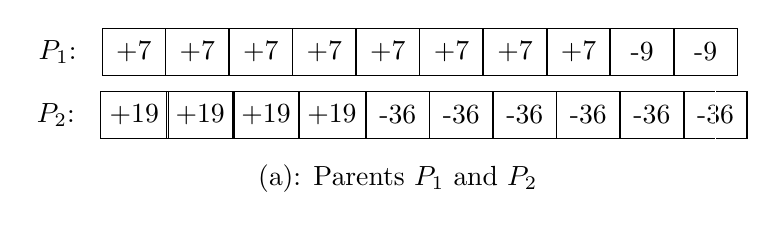
\begin{tikzpicture}
		\tikzstyle{rec} = [rectangle, minimum width=0.8cm,minimum height=0.6cm, text
		centered, draw=black]
			\node (gene11) [rec] {+7};
			\node (gene2) [rec] at ($(gene11.east)+(0.4cm,0)$)  {+7};
			\node (gene3) [rec] at ($(gene2.east)+(0.4cm,0)$)  {+7};
			\node (gene4) [rec] at ($(gene3.east)+(0.4cm,0)$)  {+7};
			\node (gene5) [rec] at ($(gene4.east)+(0.4cm,0)$)  {+7};
			\node (gene6) [rec] at ($(gene5.east)+(0.4cm,0)$)  {+7};
			\node (gene7) [rec] at ($(gene6.east)+(0.4cm,0)$)  {+7};
			\node (gene8) [rec] at ($(gene7.east)+(0.4cm,0)$)  {+7};
			\node (gene9) [rec] at ($(gene8.east)+(0.4cm,0)$)  {-9};
			\node (last) [rec] at ($(gene9.east)+(0.4cm,0)$)  {-9};
			\node[text width=1cm] at ($(gene11.west)+(-0.3cm,0)$) {$P_1$:};
			\node (gene1) [rec] at ($(gene11.east)+(-0.4cm,-0.8cm)$) {+19};
			\node (gene2) [rec] at ($(gene1.east)+(0.4cm,0)$)  {+19};
			\node (gene3) [rec] at ($(gene2.east)+(0.4cm,0)$)  {+19};
			\node (gene4) [rec] at ($(gene3.east)+(0.4cm,0)$)  {+19};
			\node (gene5) [rec] at ($(gene4.east)+(0.4cm,0)$)  {-36};
			\node (gene6) [rec] at ($(gene5.east)+(0.4cm,0)$)  {-36};
			\node (gene7) [rec] at ($(gene6.east)+(0.4cm,0)$)  {-36};
			\node (gene8) [rec] at ($(gene7.east)+(0.4cm,0)$)  {-36};
			\node (gene9) [rec] at ($(gene8.east)+(0.4cm,0)$)  {-36};
			\node (gene10) [rec] at ($(gene9.east)+(0.4cm,0)$)  {-36};
			\node[text width=1cm] at ($(gene1.west)+(-0.3cm,0)$) {$P_2$:};
			\draw[-,white] ($(gene10.north)$)-- ++(0,-1.5cm);
			\node (label1) at ($(gene5.south)+(0cm,-0.5cm)$) {(a): Parents $P_1$ and $P_2$};
		\end{tikzpicture}
}

% offspring
\resizebox{.95\linewidth}{!}{
		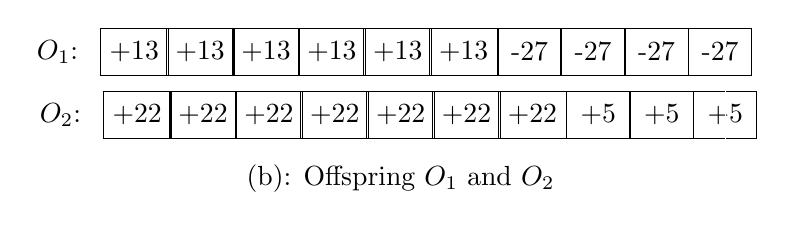
\begin{tikzpicture}
			\tikzstyle{rec} = [rectangle, minimum width=0.8cm,minimum height=0.6cm, text
			centered, draw=black]
			\node (gene11) [rec] {+13};
			\node (gene2) [rec] at ($(gene11.east)+(0.4cm,0)$)  {+13};
			\node (gene3) [rec] at ($(gene2.east)+(0.4cm,0)$)  {+13};
			\node (gene4) [rec] at ($(gene3.east)+(0.4cm,0)$)  {+13};
			\node (gene5) [rec] at ($(gene4.east)+(0.4cm,0)$)  {+13};
			\node (gene6) [rec] at ($(gene5.east)+(0.4cm,0)$)  {+13};
			\node (gene7) [rec] at ($(gene6.east)+(0.4cm,0)$)  {-27};
			\node (gene8) [rec] at ($(gene7.east)+(0.4cm,0)$)  {-27};
			\node (gene9) [rec] at ($(gene8.east)+(0.4cm,0)$)  {-27};
			\node (last) [rec] at ($(gene9.east)+(0.4cm,0)$)  {-27};
			\node[text width=1cm] at ($(gene11.west)+(-0.3cm,0)$) {$O_1$:};
			\node (gene1) [rec] at ($(gene11.east)+(-0.4cm,-0.8cm)$) {+22};
			\node (gene2) [rec] at ($(gene1.east)+(0.4cm,0)$)  {+22};
			\node (gene3) [rec] at ($(gene2.east)+(0.4cm,0)$)  {+22};
			\node (gene4) [rec] at ($(gene3.east)+(0.4cm,0)$)  {+22};
			\node (gene5) [rec] at ($(gene4.east)+(0.4cm,0)$)  {+22};
			\node (gene6) [rec] at ($(gene5.east)+(0.4cm,0)$)  {+22};
			\node (gene7) [rec] at ($(gene6.east)+(0.4cm,0)$)  {+22};
			\node (gene8) [rec] at ($(gene7.east)+(0.4cm,0)$)  {+5};
			\node (gene9) [rec] at ($(gene8.east)+(0.4cm,0)$)  {+5};
			\node (gene10) [rec] at ($(gene9.east)+(0.4cm,0)$)  {+5};
			\node[text width=1cm] at ($(gene1.west)+(-0.3cm,0)$) {$O_2$:};
			\draw[-,white] ($(gene10.north)$)-- ++(0,-1.5cm);
			\node (label1) at ($(gene5.south)+(0cm,-0.5cm)$) {(b): Offspring $O_1$ and $O_2$};
		\end{tikzpicture}
}

%mutation
\resizebox{.95\linewidth}{!}{
	\begin{tikzpicture}
	\tikzstyle{rec} = [rectangle, minimum width=0.8cm,minimum height=0.6cm, text
	centered, draw=black]
		\tikzstyle{rec} = [rectangle, minimum width=0.8cm,minimum height=0.6cm, text
		centered, draw=black]
		%\draw[help lines](-3,-3) grid (4,4);
		\node (gene11) [rec] {+13};
		\node (gene2) [rec] at ($(gene11.east)+(0.4cm,0)$)  {+13};
		\node (gene3) [rec] at ($(gene2.east)+(0.4cm,0)$)  {+13};
		\node (gene4) [rec] at ($(gene3.east)+(0.4cm,0)$)  {$\cdots$};
		\node (gene5) [rec] at ($(gene4.east)+(0.4cm,0)$)  {+13};
		\node (gene6) [rec] at ($(gene5.east)+(0.4cm,0)$)  {+13};
		\node (gene7) [rec] at ($(gene6.east)+(0.4cm,0)$)  {-27};
		\node (gene8) [rec] at ($(gene7.east)+(0.4cm,0)$)  {$\cdots$};
		\node (gene9) [rec] at ($(gene8.east)+(0.4cm,0)$)  {-27};
		\node (last) [rec] at ($(gene9.east)+(0.4cm,0)$)  {-27};
		\draw[<->,thick] (gene11.south) .. controls +(1.8,-0.4) .. (gene6.south)
			node[pos=0.5] {11} ;
		\draw[<->,thick] (gene7.south) .. controls +(1.3,-0.4) .. (last.south)
			node[pos=0.5] {7};
		\node[text width=1cm] at ($(gene11.west)+(-0.3cm,0)$) {$O_1$:};

		\node (label1) at ($(gene5.south)+(0cm,-0.8cm)$) {(c): Offspring $O_1$ after
			lenght mutation};

		\node (gene1) [rec] at ($(gene11.east)+(-0.4cm,-1.8cm)$) {+12};
		\node (gene2) [rec] at ($(gene1.east)+(0.4cm,0)$)  {+12};
		\node (gene3) [rec] at ($(gene2.east)+(0.4cm,0)$)  {+12};
		\node (gene4) [rec] at ($(gene3.east)+(0.4cm,0)$)  {$\cdots$};
		\node (gene5) [rec] at ($(gene4.east)+(0.4cm,0)$)  {+12};
		\node (gene6) [rec] at ($(gene5.east)+(0.4cm,0)$)  {+12};
		\node (gene7) [rec] at ($(gene6.east)+(0.4cm,0)$)  {-26};
		\node (gene8) [rec] at ($(gene7.east)+(0.4cm,0)$)  {$\cdots$};
		\node (gene9) [rec] at ($(gene8.east)+(0.4cm,0)$)  {-26};
		\node (last) [rec] at ($(gene9.east)+(0.4cm,0)$)  {-26};
		\node[text width=1cm] at ($(gene11.west)+(-0.3cm,0)$) {$O_1$:};
		\draw[-,white] ($(gene10.north)$)-- ++(0,-1.5cm);
		\node (label1) at ($(gene5.south)+(0cm,-0.5cm)$) {(b): Offspring $O_1$ 
			 after angle mutation};
	\end{tikzpicture}
}
\end{center}
\caption{GA Operators\label{GA:operator}}
\end{figure}

\section{Methodology}
\subsection{Objective function}
The optimization problem can be formulated by searching the optimal stacking
sequence of composite laminate.  There are two design variables here, the angles
in the laminate, and the number of layers that each fiber orientation has. The
objective function is formulated as

\begin{equation}
	\begin{split}
    	F  &= 2t_0 \sum_{k=1}^n n_k  \textstyle{,}\\
    	   &SF_{MS} \geq 1 \textstyle{,} \\
    	   &SF_{TW} \geq 1 \textstyle{.}
	\end{split} 
\end{equation}

The first term represents the total thickness of the composite laminates, $t_0$
is the ply thickness; $n_k$ is the number of plies in the kth lamina, in which
the fiber orientation is $\theta_k$. The constraints here are two safety
factors should not less than 1, which means  $SF_{MS} \geq 1$, and $SF_{TW} \geq
1$, respectively.

\subsection{Encoding}
Due to the simplicity and efficiency of float representation, this encoding
method is implemented to represent a possible solution. As shown in Figure \ref{GA:operator}
 (a), these two chromsomes represent a $[+8_{7}/-9_{2}]_s$
carbon T300/5308 laminated composite, and $[+19_{4}/-36_{6}]_s$, respectively.
Becasue the laminate adopted in this paper is symmetric to its mid-plane, so
only half needs to be encoded.

\subsection{Selection}
The purpose of the selection operator is to choose mating pool to produce
alternative solutions of better fitness. Traditional methods of selecting
strategies only take the fitness of individuals into account, however, due to 
the existence of constraint, various selection schemes are implemented to
select the mating set. Based on different selection schemes, the parents of
next generation can be divided into  three groups: proper groups, active groups,
and potential groups according to different selecting methods. 

Proper parents mean in which individual fullfills the constraints, which are
chosen by the individual's fitness, individuals with better fitness are more
likely to be chosen if they fit the constraint; active group means that
individual within this group is supposed to always exist in the parents during the GA, which
are selected by fitness, ignoring the constraint; The individuals from the active
group may not correspond to feasible solutions, but their existence enriches the
variety of the gene clips.  Potential group means that individuals are likely to turn
into proper individual after a couple of generations, and potential individuals
are chosen by constraint function, the more the individual fulfills the
constraint, the more possibility it will be selected.

\subsection{Crossover}
The crossover operator happens among these three groups. the child of two proper
groups is more likely to be a proper individual which can be used to obtain an
alternative feasible solution. the child of an active individual and a potential
individual can significantly change the gene of an active individual's chromosome,
which makes the individual evolve toward a new direction. The offspring of two
active individuals are more likely to be an active individual, which can maintain
the active group.  The figure.\ref{GA:operator} (b) shows two children $O_1$
and $O_2$ from two parents $P_1$ and $P_2$, each angle $C_a$ and its length 
$C_l$ of a child are obtained by the following formula
\begin{align} 
	\begin{cases}
	C_a &= (P1_a + P2_a)/2 \\
	C_l &= (P1_l + P2_l)/2 
\end{cases} \textstyle{.}
\end{align}
\begin{table}[tb]
\caption{Comparison of the carbon/epoxy, graphite/epoxy, and glass/epoxy properties}
\centering
\begin{adjustbox}{width=0.5\textwidth}
\label{tab:mat}
\begin{tabular}{lccccc}
\toprule
Property								   & Symbol				  & Unit  &  Carbon/Epoxy&  Graphite/Epoxy  &  Glass/Epoxy   \\
\midrule
Longitudinal elastic modulus			   & $E_1$				  & GPa   &  116.6       &  181             &  38.6           \\
Traverse elastic modulus				   & $E_2$				  & GPa   &  7.67        &  10.3            &  8.27           \\
Major Poisson's ratio					   & $v_{12}$			  &       &  0.27        &  0.28            &  0.26           \\
Shear modulus							   & $G_{12}$			  & GPa   &  4.17        &  7.17            &  4.14           \\
Ultimate longitudinal tensile strength     & $(\sigma_1^T)_{ult}$ & MP    &  2062        &  1500            &  1062            \\
Ultimate longitudinal compressive strength & $(\sigma_1^C)_{ult}$ & MP    &  1701        &  1500            &  610             \\
Ultimate transverse tensile strength       & $(\sigma_2^T)_{ult}$ & MPa   &  70          &  40              &  31              \\
Ultimate transverse compressive strength   & $(\sigma_2^C)_{ult}$ & MPa   &  240         &  246             &  118              \\
Ultimate in-plane shear strength           & $(\tau_{12})_{ult}$  & MPa   &  105         &  68              &  72               \\
Density                                    & $\rho$               & $g/cm^3$ &  1.605    &  1.590           &  1.903               \\
Cost                                       &                      &       &  8           &  2.5             &  1               \\
\bottomrule
\end{tabular}
\end{adjustbox}
\end{table}

\subsection{Mutation}
A mutation direction is imposed on the mutation operator which to make sure the
individual evolving toward the right direction. The mutation direction, denoted
by $md$, is an n dimensional vector corresponding to the number of constraints, it
is decided by the constraint thresholds $CT_i$ and the current individual's
constraint value, denoted as $CV_i$,  The mutation vector can be obtained by the
following formula

\resizebox{.9\linewidth}{!}{
	$\text{md} = [CT_1, \cdots, CT_{n-1}, CT_n] -  [CV_0, \cdots, CV_{n-1}, CV_n] \textstyle{.}$

}

During this operator, the mutation procedure is consist of two phases: the length
mutation of the chromosome, and the angle mutation of the chromosome.  Because the
chromosome's length is positively correlated with the individual's fitness, the
coefficient of length mutation denoted by $C_l$, if $\sum_{i=1}^{N}{CT_i}$ great
than $\sum_{i=1}^{N}{CV_i}$ , the mutation length is restricted to the range
$[0,(C_l \sum_{i=1}^{N}{(CT_i-CV_i)})/N]$, which means increase the chromosome's
length; Assuming a $[+13_6/-27_4]_s$ T300/5308 carbon/epoxy composite
laminate under the loading $N_{x} = N_{y} = 10$ MPa m, it's property as shown
in table \ref{tab:T300/5308}. According to CLT and
failure theory, the two safety factors $SF_{MS}$ and $SF_{TW}$ are  0.0539, and
0.0540, respectively. So the mutation vector and is $[0.9461,0.9460]$, assuming
the length mutation coefficient is 20, so the mutation range is from 0 to 18. A
random number is generated from the range $[0, 18]$, supposing the outcome is
13, then a length generator is used to a list, the its sum is 13, suppose the
list is [5, 8], the laminate after mutation is $[13_{11}/-27_{12}]_s$.

If the $\sum_{i=1}^{N}{CT_i}$ less than $\sum_{i=1}^{N}{CV_i}$, the
mutation length is restricted to the range $([\sum_{i=1}^{N}{CT_i-CV_i})/N,0]$,
which means the individual's fitness exceeds the threshold value, and decrease
the chromsome's length.  Assuming a $[+33_{35}/-29_{26}]_s$ T300/5308 laminate
is under loading $N_{x}=10$ MPa, and $N_{y}=5$ MPa, then, it's $SF_{MS}$
constraint and $SF_{TW}$ values are  1.0912, 1.0747, respectively.
because the length mutation is 20, so the mutation range is from -2 to 0. This
would decrease the chromosome's length. 
\begin{align}
	\text{LM} = 
	\begin{cases}
		\resizebox{.35\textwidth}{!}{$[0,(C_l \sum_{i=1}^{N}{(CT_i-CV_i)})/N], \text{ if }  \sum_{i=1}^{N}{CT_i} > 
		\sum_{i=1}^{N}{CV_i}$}\\
		\resizebox{.35\textwidth}{!}{$[(C_l \sum_{i=1}^{N}{(CT_i-CV_i)})/N,0], \text{ if }  \sum_{i=1}^{N}{CT_i} < 
		\sum_{i=1}^{N}{CV_i}$}\\
	\end{cases} 
\end{align}

The relationship between the angles in the composite laminate and the
chromosome's fitness is unclear, so the mutation direction of chromosome's angle
is random. The coefficient angle mutation is $C_a$, the angle mutation range is
$[0,C_a \sum_{i=1}^{N}{(|CT_i-CV_i|)}]$ or $[C_a
\sum_{i=1}^{N}{(-|CT_i-CV_i|)},0]$. It is can be written as

\begin{align}
	\text{P(AM)} =  
	\begin{cases}
		0.5, \text{ AM = }[0,C_a \sum_{i=1}^{N}{(|CT_i-CV_i|)}] \\ 
	    0.5, \text{ AM = }[C_a \sum_{i=1}^{N}{(-|CT_i-CV_i|)},0]
	\end{cases} \textstyle{.}
\end{align}

\section{Result and Discussion}
We have conducted experiment by the use of the generated data set. This data
set is randomly partitoned into a training set and a test.

Figure \ref{fig:train-process} shows five ANNs with different topologies, quite
different results have been observed when different architectures are adopted.
It is clear that architecture whose mean of average difference is less than the
rest.


\begin{figure}
	\centering
	\def\svgwidth{\columnwidth}
	\import{fig/}{pre_train.pdf_tex}
	\label{fig:train-process}
\end{figure}

Table \ref{tab:simu} shows part of the valudation.
\begin{table}[!tb]
	\centering
	\caption{ANN predictions of the Tsai-wu and MS strength ratio with the
	numberical results obtained by CLT.}
	\label{tab:simu}
	\begin{adjustbox}{width=0.5\textwidth}
	\begin{tabular}{cccc|cc|cc}
		\toprule
		\multicolumn{4}{c}{\textbf{Input}} &  \multicolumn{4}{c}{\textbf{Output}} \\
		\midrule
		Load  &  \makecell{Laminate \\ Structure }  & \makecell{Material \\ Property} & \makecell{Failure \\  Property}  &
		\multicolumn{2}{c}{ \makecell {CLT \\MS  Tsai-Wu}} & \multicolumn{2}{c}{ \makecell {ANN \\MS  Tsai-Wu}}\\
		\midrule
		-10,40,20  &  26,-26,168,1.27 & 116.6,7.67,0.27,4.17 & 2062.0,1701.0,70,240,105 & 0.342 & 0.476 & 0.351 & 0.492 \\
		20,-70,-30 &  10,-10,196,1.27 & 181.0,10.3,0.28,7.17 & 1500.0,1500.0,40,246,68  & 0.653 & 0.489 & 0.612 & 0.445 \\ 
		60,-20,0   &  82 -82,128,1.27 & 181.0,10.3,0.28,7.17 & 1500.0,1500.0,40,246,68  & 1.663 & 0.112 & 1.673 & 0.189 \\
		\bottomrule
	\end{tabular}
	\end{adjustbox}
\end{table}



\begin{figure}
	\centering
	\def\svgwidth{\columnwidth}
	\import{fig/}{post_train.pdf_tex}
	\label{fig:final_train}
\end{figure}


Comparing the strength ratio outputs based on CLT and ANN from
Tab.\ref{tab:simu}, we can see that the calculation of strength ratio can be
achieved using a two-layer neural network, without the intensive computation of
matrix multiplication.





\section{Conclusion}
In this paper, an evolutionary artificial neural network model was developed to
predict the strength ratio of laminated composite material under in-plane
loading. We review the use of genetic algorithms and artificial neural networks
as an alternative approach for calculating the strength ratio of an angle ply
laminate under in-plane loading. Traditionally, it is obtained through CLT and
corresponding failure criteria, such as Maximum Stress theory and Tsai-Wu
failure theory.

The main contribution of this work is as follows: 1) propose a two-layer diagram
model for designing a sophisticated neural network in simulating the calculation
of strength ratio, and use a genetic algorithm to explore the search space. 2)
suggest an efficient method to compute the strength ratio instead of adopting
the two-step procedure based on classical lamination theory and related failure
criteria. Compared with experimentally obtained data, it is demonstrated that
ANN is an efficient and simple tool to compute the strength ratio, instead of
the complex analytical mathematical model. Our findings underline the practical
applicability of ANN on the analysis of composite material.

There are more improvements we can make over the search strategy and application
in the area of laminated composite material. The future work is to develop a
more sophisticated ANN, which not only can predict the properties for angle ply
laminate, but also the other type of laminated composite material.


\section{Acknowledgment}
The paper is based on the work supported by China Scholarship Council with
the code number 201806630112


\bibliographystyle{plain}
\bibliography{src/a6_reference}

\end{document}
